%% Introduce what sequencing machines are in the context
 Mapping DNA has become possible with the democratisation of \emph{sequencing machines} or \emph{sequencers}. The first sequencer was released in 1986, making it a rather recent invention. These machines take a DNA sample and find the sequences of A, T, C and G bases from it. The latest ones are called \emph{third generation sequencers}, and are remarkable for their long sequences reads of more than 5000 bases and their ability to compensate for their low raw read precision with prediction algorithms~\cite{Lee048603}. Different technologies exist depending on the machine manufacturer. For example, one technique involves using a nanopore as an electrical sensor with a hole through which the DNA string passes, much like a sensor reading a cassette tape. The ionic composition of each base creates a different current change in the sensor, making it possible to deduce which nucleotide it is~\cite{Oxford:nanopore}.

In this thesis, we focus on Next Generation Sequencing (NGS) with Illumina sequencing machines. Their technology for sequencing is called "Sequencing by Synthesis"~\cite{illumina:sbs}. All steps are summarised in Figure~\ref{fig:sbs}. First, DNA is broken into small pieces of 200 to 600 bases pairs called fragments during the sample preparation phase. At the end of each fragment, special molecules called adapters are added to give each fragment an index, and a binding site for the rest of the process. Each fragment is attached by one of its ends to a substrate, the flow cell. It is replicated by bending over, attaching its other end to the substrate, and letting a polymerase create the complement of each base (pairing A with T, T with A, C with G and G with C), then washing away the reverse-complement strand newly created. This is the cluster generation phase. By bending over, creating the complement, then washing it away, the direct strand is replicated millions of times. The direct strand is then sequenced by sending particular DNA nucleotides that have a photosensitive end. After being attached, they are excited by a laser, and the attached base emits a wavelength characteristic of the base (A, T, C or G). The colour of the emitted light is captured by a camera to deduce the base attached. The reverse strand is then created by complementing the direct strand. With another cluster generation phase, millions of copies of the reverse strand are created, and sequenced using the same photosensitive bases. Illumina machines output both the forward and reverse reads, which are called pair-end reads.

\begin{figure}
    \centering
    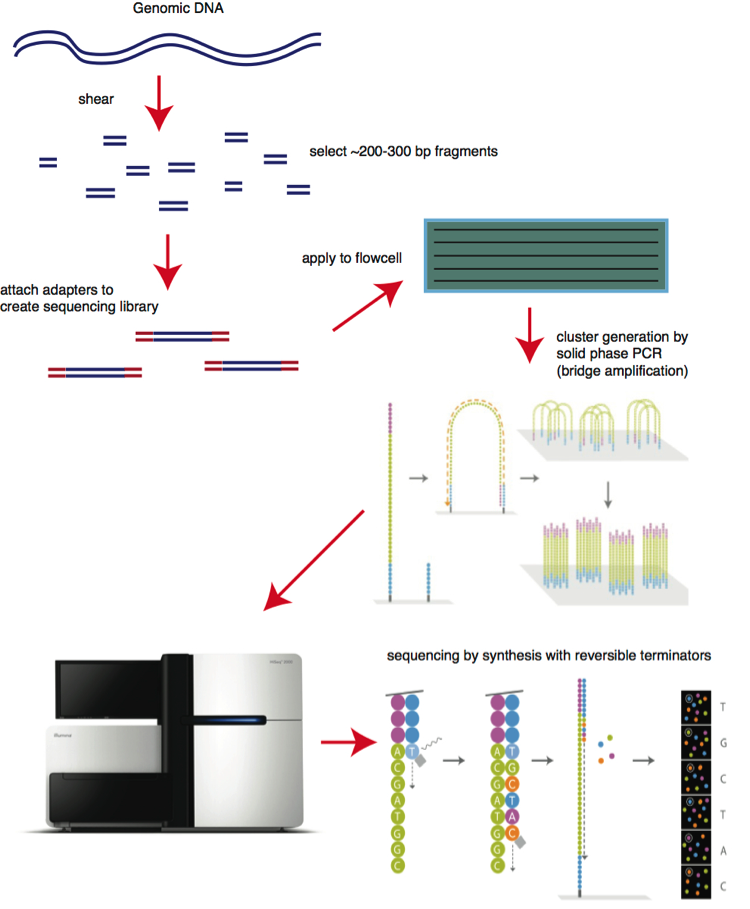
\includegraphics{sbs}
    \caption{Sequencing by Synthesis process for Illumina sequencers. (from~\cite{bitesizebio:sbs}}
    \label{fig:sbs}
\end{figure}{}

This process generates millions of pair-end reads, representing all the fragments. These fragments have to be mapped to a reference genome to deduce information about the sample they come from.

Read sequences and the reference genome are composed of nucleotides or bases, which are reported from their first letter: A, T, C and G. First, we need to introduce the fact that the alignment should provide some kind of metric, to quantify how good the alignment is. Basically, this metric should be a score that increases when there is very few to no differences between the two string of characters, and decreases if they differ, so when letters are not matching. In the case of DNA, mutations often take the form of adding bases, deleting bases, or changing some bases, as seen on Figure~\ref{fig:mutation}, so the meaning of the score value should reflect these mutations.

\begin{figure}[h!]
	\centering
	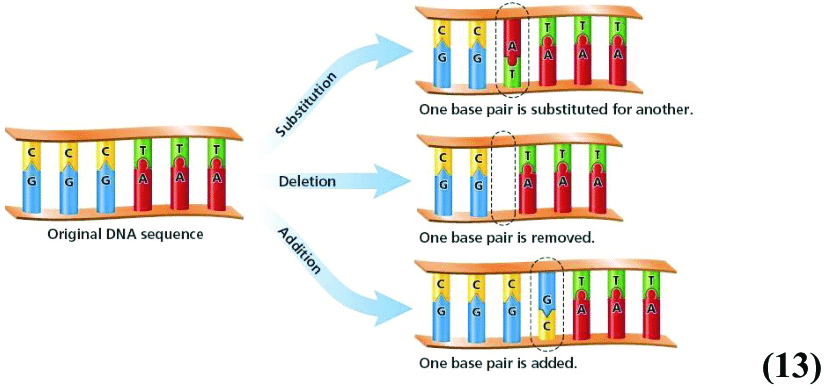
\includegraphics[width=0.7\linewidth]{mutation}
	\caption{Examples of mutation (from~\cite{alasadi:chemistry})}
	\label{fig:mutation}
\end{figure}

Another challenge is to process a huge number of sequences as fast as possible. In fact, DNA sequencers produce strings of a given length proper to each machine. While older sequencers produce short strings of 80 or 150 bases, more recent ones can output several thousand of bases per string, and millions of strings are produced. These strings are not related to each other, hence, there is no obstacle in processing multiple of them at the same time. This mode is called \emph{inter-sequence parallelisation}. It is also possible to parallelise the alignment calculation for each sequence, but this mode, named \emph{intra-sequence parallelisation}, requires extra care about synchronisation.

% Furthermore, looking into a full genome for a match would be an incredibly tedious task without an efficient search algorithm. It is then advisable to create an index of the reference genome. With this index, operations to research a given pattern in a huge data set can be faster than linear time with respect to the data size.

